\documentclass[12pt, twoside]{article}
\usepackage[letterpaper, margin=1in, headsep=0.5in]{geometry}
\usepackage[english]{babel}
\usepackage[utf8]{inputenc}
\usepackage{amsmath}
\usepackage{amsfonts}
\usepackage{amssymb}
\usepackage{tikz}
\usepackage{yhmath}
%\usetikzlibrary{quotes, angles}

\usepackage{graphicx}
\usepackage{enumitem}
\usepackage{multicol}

\usepackage{fancyhdr}
\pagestyle{fancy}
\fancyhf{}
\renewcommand{\headrulewidth}{0pt} % disable the underline of the header

\fancyhead[RE]{\thepage}
\fancyhead[RO]{\thepage \\ Name: \hspace{3cm}}
\fancyhead[L]{BECA / Dr. Huson / 10th Grade Geometry\\* 30 January 2020}

\begin{document}
\subsubsection*{8.3 Do Now: Density}
 \begin{enumerate}

  \item A pentagon is inscribed in circle $O$, as shown below. The circle has radius $r=10$.
    \begin{multicols}{2}
    \raggedcolumns
    \begin{enumerate}
      \item Find the area of the sector $AOB$. \vspace{3cm}
      \item Find the perimeter of the sector $AOB$. %\vspace{1.5cm}
    \end{enumerate}
      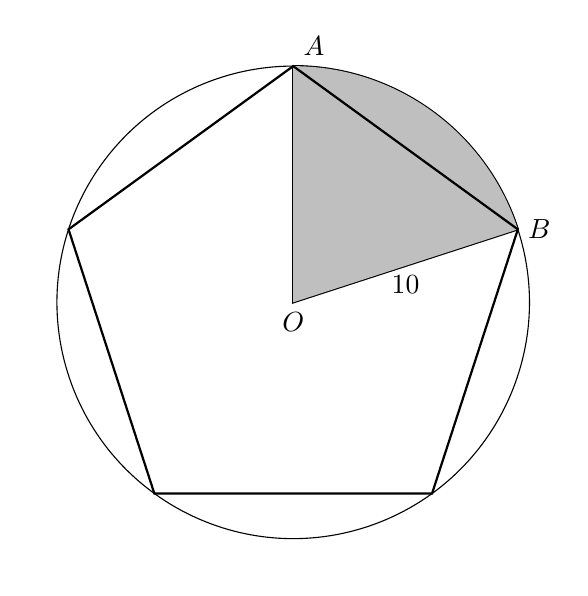
\begin{tikzpicture}[scale=1, rotate=18]
        \draw (0,0) circle[radius=3];
        \draw [thick]
        (0:3) node[right] {$B$}--
        (0,0) node[below] {$O$}--
        (72:3) node[above right] {$A$} arc (72:0:3);
        \fill [lightgray]
        (0,0)--(0:3) arc (0:72:3)--(0,0);
        \draw (1.5,0) node[below] {$10$};
        \draw [thick] (0:3)--(72:3)--(2*72:3)--(3*72:3)--
        (4*72:3)--cycle;
      \end{tikzpicture}
    \end{multicols}  \vspace{1cm}

  \item A cylinder is 12.3 cm tall and has a volume of 966 cubic cm. Find the area of the base of the cylinder. Express your result to the \emph{nearest hundredth of a square centimeter}. \vspace{3cm}

  \item Find the area of the shape shown below composed of a rectangle and a semi-circle.
  \begin{flushright}
  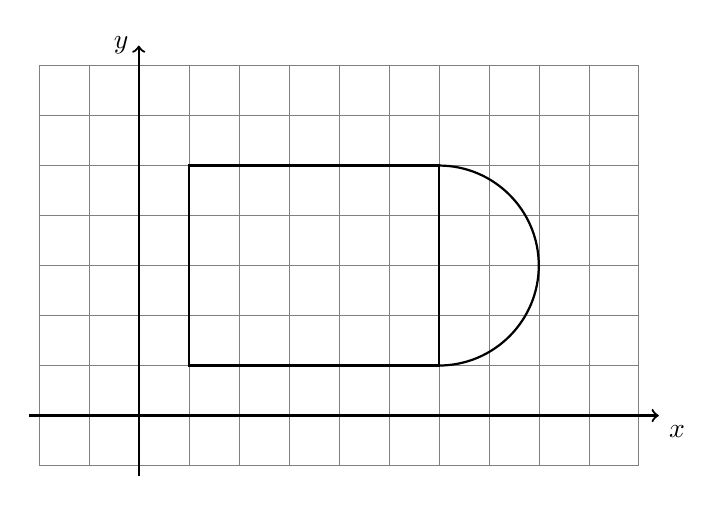
\begin{tikzpicture}[scale=.635]
    \draw [help lines] (-2,-1) grid (10,7);
    \draw [thick, ->] (-2.2,0) -- (10.4,0) node [below right] {$x$};
    \draw [thick, ->] (0,-1.2)--(0,7.4) node [left] {$y$};
    \draw [thick] (1,1)--(6,1)--(6,5)--(1,5)--cycle;
    \draw [thick] (6,1) arc (-90:90:2);
  \end{tikzpicture}
\end{flushright}

\newpage
\subsubsection*{Estimating and measuring}

  \item The diagram below shows $\triangle ABC$, with $\overline{AEB}$, $\overline{ADC}$. $AB=12$, $AD=6$. Estimate $BC$, assuming that the diagram below is drawn to scale.
  \begin{multicols}{2}
    Write the actual lengths of 
    \begin{enumerate}
      \item $AB=$ \vspace{0.7cm}
      \item $AD=$ \vspace{0.7cm}
      \item $BC=$  \vspace{0.7cm}
      \item Find the scale factor, $k$ \vspace{1.2cm}
      \item Calculate $BC=$
    \end{enumerate}
      \begin{tikzpicture}[scale=1.5]
        \draw [thick]
        (0,0) node[above right] {$A$}--
        (230:6) node[below left] {$B$}--
        (260:4.75) node[below right] {$C$}--cycle;
        \draw [thick]
        (230:2.375) node[above left] {$E$}--
        (260:3) node[right] {$D$}--cycle;
      \end{tikzpicture}
    \end{multicols}\vspace{2cm}

  \item Given the circle with center $P$ with central angle $\angle APB$ and inscribed angle $\angle AQB$. Using a protractor, measure each angle.
  \begin{multicols}{2}
    \raggedcolumns
    \begin{enumerate}
      \item $m\angle APB=$ \vspace{0.7cm}
      \item $m\angle AQB=$ \vspace{0.7cm}
      \item What do you think is the ratio of the central angle to the inscribed angle?
    \end{enumerate}
      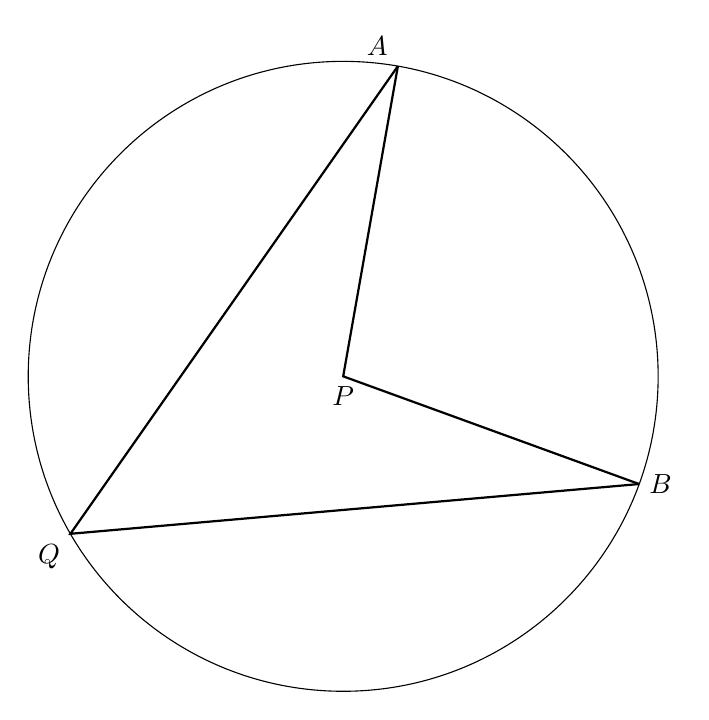
\begin{tikzpicture}[scale=.8]
        \draw (0,0) circle[radius=5];
        \draw [thick]
        (-20:5) node[right] {$B$}--
        (0,0) node[below] {$P$}--
        (80:5) node[above left] {$A$};
        \draw [thick] (-20:5)--(210:5) node[below left] {$Q$}--(80:5);
        %\draw (60:5) node[right]{$130^\circ$};
      \end{tikzpicture}
  \end{multicols}

\newpage
\subsubsection*{Applying density ratios}
\item Find the weight of a metal block with a volume of 20 cubic inches and a density of 0.75 pounds per cubic inch. \vspace{3cm}
\item A large block of ice has a volume of 45 liters. The density of ice (water) is one kilogram per liter. Find the weight of the ice.  \vspace{3cm}
\item A tank of gasoline holds 20 gallons. Find the cost to completely fill the tank if gasoline costs \$2.35 per gallon. \vspace{3cm}
\item A bar of solid gold is in the shape of a rectangular prism having a length of 10 cm, width of 4 cm, and thickness of 1.5 cm. The density of gold is 19.3 grams per cubic cm, and its approximate market value is \$50 per gram.
\begin{enumerate}
  \item Find the weight of the bar of gold.  \vspace{3cm}
  \item Find its value in dollars.
\end{enumerate}

\newpage
\subsubsection*{Vocabulary self-assessment: Circles (fill in the blank with the correct term)}

  \item \textbf{Internal line segments:} Circle with center at point $P$, as shown.
    \begin{multicols}{2}
      \begin{itemize}
        \item  $\overline{AB}$ \quad \rule{3cm}{0.15mm} %Diameter
        \item  $\overline{CP}$ \quad \rule{3cm}{0.15mm} %Radius
        \item  $\overline{DE}$ \quad \rule{3cm}{0.15mm} %Chord
        \item $\angle APC$ \quad \rule{3cm}{0.15mm} %Central angle 
        \item  $\wideparen{AC}$ \quad \rule{3cm}{0.15mm} %(with measure $m\wideparen{AC} = 72^\circ$)Arc
      \end{itemize}
    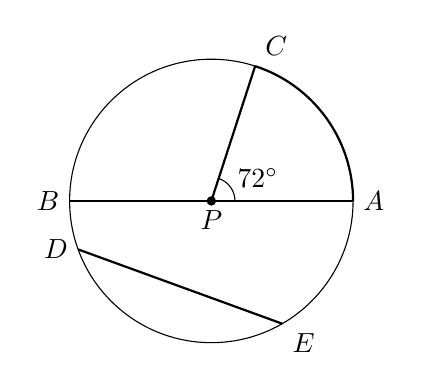
\begin{tikzpicture}[scale=0.6]
      \draw (0,0) circle[radius=3];
      \draw [thick] (3,0) arc (0:72:3);
      \draw [thick] (0:3) node[right] {$A$}--(180:3) node[left] {$B$};
      \draw [thick] (0,0)--(72:3) node[above right] {$C$};
      \draw [thick] (200:3) node[left] {$D$}--(300:3) node[below right] {$E$};
      \fill (0,0) circle[radius=0.1] node[below]{$P$};
      \draw (0.5,0) arc (0:72:0.5) node[right]{$\ 72^\circ$};
      %\draw (35:5) node[right] {$\wideparen{AC}$};
      %\draw (290:5) node[below] {$D$};
    \end{tikzpicture}
  \end{multicols}

  \item \textbf{External lines:} Circle with center at point $O$, at right.
    \begin{multicols}{2}
      \begin{itemize}
        \item  $\overline{FGH}$ \quad \rule{3cm}{0.15mm} %Secant
        \item  $\overline{OJ}$ \quad \rule{3cm}{0.15mm} %Radius
        \item  $\overline{FJK}$ \quad \rule{3cm}{0.15mm} %Tangent
        \item $J$ \quad \rule{3cm}{0.15mm} %Point of tangency 
        %\item Note: $\overline{OJ} \perp \overline{FJK}$
      \end{itemize}
    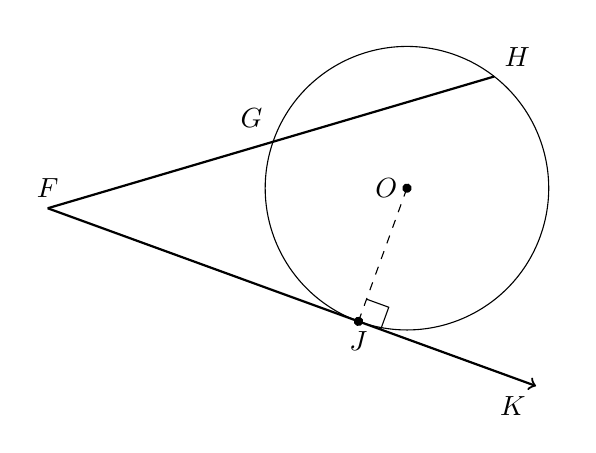
\begin{tikzpicture}[scale=0.6, rotate=-20]
      \draw (0,0) circle[radius=3];
      \draw [thick, ->] (-7,-3) node[above] {$F$}--(4,-3) node[below left] {$K$};
      \draw [thick] (-7,-3)--(72:3) node[above right] {$H$};
      \draw [dashed] (0,-3) node[below] {$J$}--(0,0);
      \fill (0,0) circle[radius=0.1] node[left]{$O$};
      \fill (0,-3) circle[radius=0.1];
      \draw (0,-3) ++(0.5,0)-- ++(0,0.5)--++(-0.5,0);
      \draw (170:3.8) node[below] {$G$};
    \end{tikzpicture}
  \end{multicols}
    
  \item \textbf{Areas:} Circle with center at point $Q$.
    \begin{multicols}{2}
      \begin{itemize}
        \item  $\overline{RS}$ \quad \rule{3cm}{0.15mm} %Diameter
        \item  $RST$ \quad \rule{3cm}{0.15mm} %Semi-circle
        \item  $QUV$ \quad \rule{3cm}{0.15mm} %Sector
      \end{itemize}
    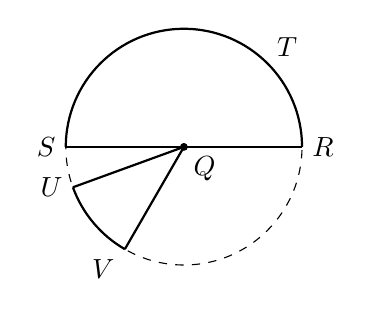
\begin{tikzpicture}[scale=0.5]
      \draw [dashed](0,0) circle[radius=3];
      \draw [thick] (0,0) ++(3,0) arc (0:180:3);
      \draw [thick] (200:3) arc (200:240:3);
      \draw [thick] (0:3) node[right] {$R$}--(180:3) node[left] {$S$};
      \draw [thick] (0,0)--(200:3) node[left] {$U$};
      \draw [thick] (0,0)--(240:3) node[below left] {$V$};
      \fill (0,0) circle[radius=0.1] node[below right]{$Q$};
      \draw (50:3.3) node[right] {$T$};
    \end{tikzpicture}
  \end{multicols}

  \begin{multicols}{2}
  \item \textbf{Polygons and angles in circles:} %Circle with triangle inscribed.
      \begin{itemize}
        \item  $\triangle XYZ$ \vspace{0.5cm} \quad \rule{3cm}{0.15mm} %Inscribed
        \item  $\angle XYZ$ \quad \rule{3cm}{0.15mm} %Inscribed
      \end{itemize} \hspace{1cm}
    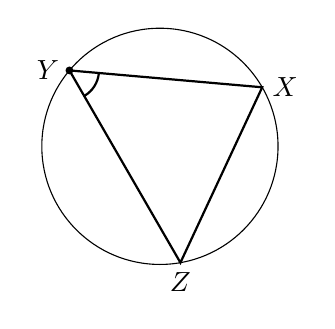
\begin{tikzpicture}[scale=0.5]
      \draw (0,0) circle[radius=3];
      \draw [thick] (140:3) ++(-60:0.75) arc (-60:-5:0.75);
      \draw [thick] (30:3) node[right] {$X$}--(140:3) node[left] {$Y$}
      --(280:3)node[below] {$Z$}--cycle;
      %\draw [thick] (0,0)--(200:3) node[left] {$U$};
      %\draw [thick] (0,0)--(240:3) node[below left] {$V$};
      \fill (140:3) circle[radius=0.1];
      %\draw (50:3.3) node[right] {$T$};
    \end{tikzpicture}
  \end{multicols}

\end{enumerate}
\end{document}
